
\begin{figure}[t!]
	\centering
	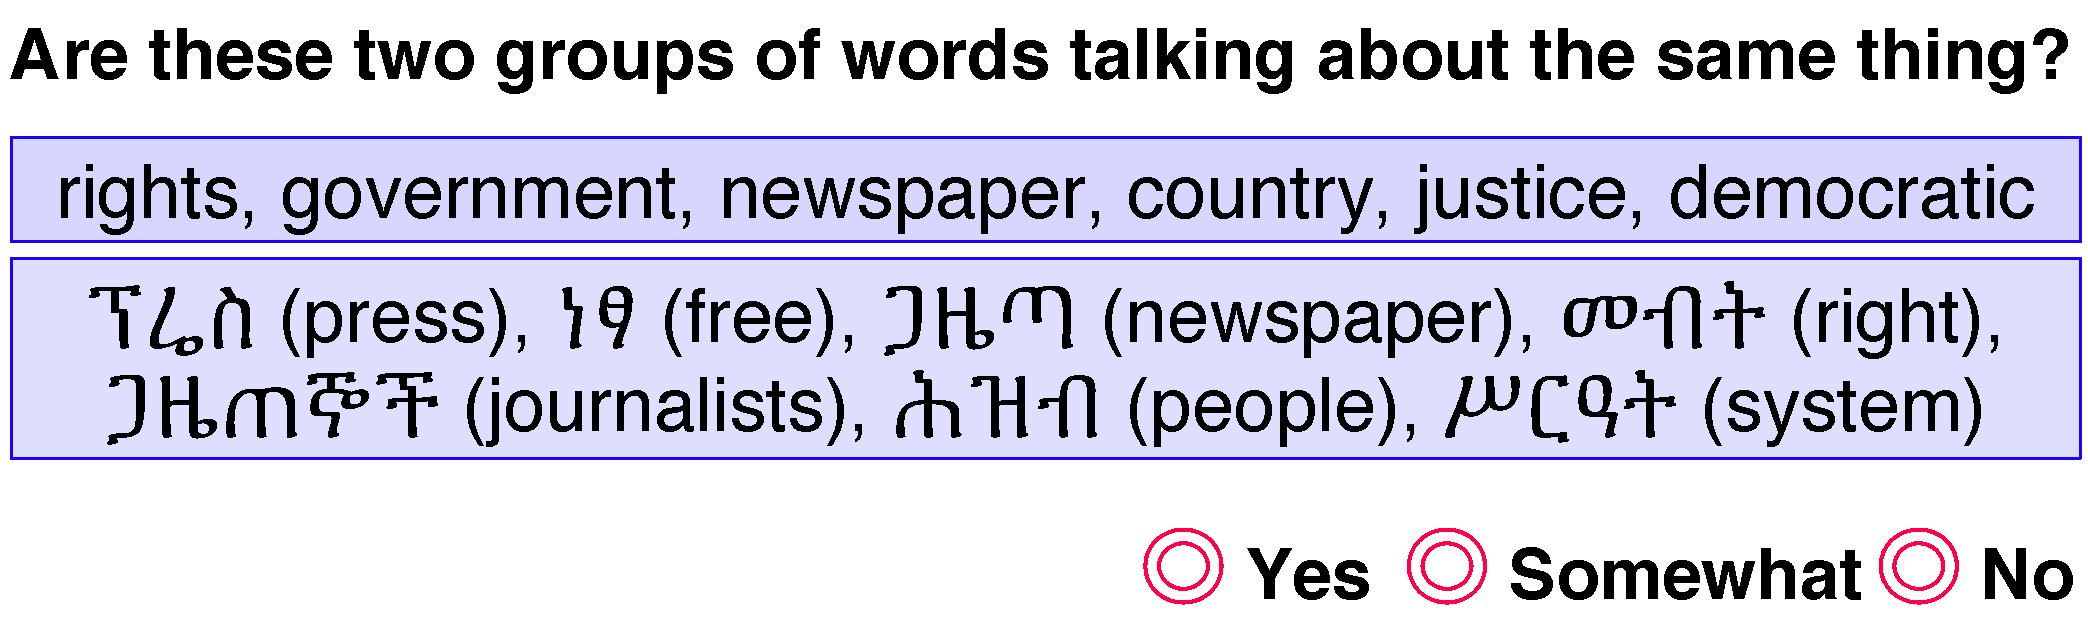
\includegraphics[width=0.48\textwidth]{2018_naacl_mltm_eval/figures/interface.pdf}
	\caption{The interface for topic quality judgments. Users read
		the topic first, and make a judgment on whether the words in
		this pair are talking about the same thing. The translations
		are here for illustration; they are not shown to the users.}
	\label{human-inter}
\end{figure}


\section{Topic-Level Evaluation}
\label{sec:topic-level}


We first study \cnpmi{} at the topic level: does a particular topic make
sense?  An effective evaluation should be consistent with
human judgment of the topics~\cite{ChangBGWB09}. In this section, we measure gold-standard
human interpretability of multilingual topics to
establish which automatic measures of topic interpretability work best.


\begin{table}[t!] \centering
	\small
	\setlength\tabcolsep{5pt}
	\begin{tabular}{c|rr|rr|c}
		\hline
		& \multicolumn{2}{c|}{Wikipedia} & \multicolumn{2}{c|}{The Bible} & \multirow{2}{*}{\textsc{mta}} \\ \cline{2-5}
		& \cnpmi{} & \inpmi{} &  \cnpmi{} & \inpmi{} & \\ \hline\hline
		\textsc{en-ro} & $0.490$ & $0.118$ & $-0.096$ & $0.031$ & $\bm{0.592}$ \\
		\textsc{en-sv} & $\bm{0.453}$ & $-0.295$ & $0.164$ & $-0.351$ & $0.248$ \\
		\textsc{en-am} & $0.110$ & $0.019$ & $\bm{0.289}$ & $0.249$ & $0.172$ \\
		\textsc{en-tl} & $\bm{0.512}$ & $0.277$ & $0.166$ & $0.002$ & $0.289$ \\
		\textsc{en-tr} & $0.664$ & $0.243$ & $0.209$ & $-0.246$ & $\bm{0.677}$ \\
		\textsc{en-zh} & $\bm{0.436}$ & $0.297$ & $0.274$ & $0.157$ & $0.411$ \\ \hline
	\end{tabular}
	\caption{Pearson correlations between human judgments and \cnpmi{} are higher than \inpmi{}, while \mta{} correlations are comparable to \cnpmi{}.}
	\label{tab:hj-table}
\end{table}



\subsection{Task Design}

Following monolingual coherence evaluations~\cite{LauNB14}, we present
topic pairs to bilingual CrowdFlower users.  Each task is a topic pair
with the top ten topic words ($C=10$) for each language.  We ask if
both languages' top words in a multilingual topic are talking about
the same concept (Figure~\ref{human-inter}), and make a judgment on a
three-point scale---coherent (2 points), somewhat coherent (1 point),
and incoherent (0 points). To ensure the users have adequate language
competency, we insert several topics that are easily identifiable as
incoherent as a qualification test.

We randomly select sixty topics from each language pair ($360$ topics
total), and each topic is judged by five users. We take the average
of the judgment points and calculate Pearson correlations with
the proposed evaluation metrics (Table~\ref{tab:hj-table}). \npmi{}-based
scores are separately calculated from each reference corpus.


\begin{table}[t!]

	\centering
	\small
		\centering
		\begin{tabular}{crccc}
			\hline
			\textbf{Test} & \textbf{Bible} & \multicolumn{3}{c}{\textbf{Train}} \\ \hline\hline
			& & \textsc{ro+sv} & \textsc{zh+tr} & \textsc{ro+sv+zh+tr} \\  \cline{3-5}
			\textsc{am} &  $-0.015$ & $0.332$ & $0.315$ &  $0.333$ \\
			\textsc{tl} &  $-0.309$ & $0.767$ & $0.631$ &  $0.705$ \\ \hline
			& & \textsc{am+tl} & \textsc{zh+tr} & \textsc{am+tl+zh+tr} \\  \cline{3-5}
			\textsc{ro} &  $-0.269$ & $0.736$ & $0.681$ &  $0.713$ \\
			\textsc{sv} &  $0.000$ & $0.787$ & $0.645$ &  $0.683$ \\ \hline
			& & \textsc{ro+sv} & \textsc{am+tl} & \textsc{ro+sv+am+tl} \\  \cline{3-5}
			\textsc{zh} &  $0.217$ & $0.751$ & $0.732$ &  $0.741$ \\
			\textsc{tr} &  $0.113$ & $0.680$ & $0.642$ &  $0.666$ \\ \hline
		\end{tabular}
	\caption{Correlations between the
          Wikipedia-based \cnpmi{} and the Bible-based \cnpmi{},
          before and after using the coherence estimator, at the topic level. Strong
          correlations indicate that the estimator improves \cnpmi{}
          estimates.}
	\label{tab:est-topic}
\end{table}


\subsection{Agreement with Human Judgments}

\cnpmi{} (the extended metric) has higher correlations with human
judgments than \inpmi{} (the naive adaptation of monolingual \npmi{}),
while \mta{} (matching translation accuracy) correlations are
comparable to \cnpmi{}.



Unsurprisingly, when using Wikipedia as the reference, the
correlations are usually higher than when using the Bible. The Bible's
archaic content limits its ability to estimate human judgments in
modern corpora (Section~\ref{sec:coherence-estimator}).

Next, we compare \cnpmi{} to two baselines: \inpmi{} and \mta{}. As
expected, \cnpmi{} outperforms \inpmi{} regardless of reference corpus
overall, because \inpmi{} only considers monolingual coherence. \mta{}
has higher correlations than \cnpmi{} scores from the Bible, because the
Bible fails to give accurate estimates due to limited topic
coverage. \mta{}, on the other hand, only depends on dictionaries,
which are more comprehensive than the Bible. It is also possible that 
users are judging coherence based on
translations across a topic pair, rather than the overall coherence,
which would closely correlate with \mta{}.






\subsection{Re-Estimating Topic-Level Coherence}
\label{sec:estimator}

The Bible---by itself---produces \cnpmi{} values that do not correlate
well with human judgments (Table~\ref{tab:hj-table}).  After
training an estimator (Section~\ref{sec:est-train}), we calculate 
Pearson's correlation between Wikipedia's \cnpmi{} and the estimated
topic coherence score (Table~\ref{tab:est-topic}).  A higher
correlation with Wikipedia's \cnpmi{} means more accurate coherence.

As a baseline, the correlation of Bible-based \cnpmi{} without
adaptation has negative and near-zero correlations with
Wikipedia;\footnote{Normally one would not estimate \cnpmi{} on
  rich-resource languages using low-resource languages. For
  completeness, however, we also include these situations.}  it does
not capture coherence.  After training the estimator, the correlations
become stronger, indicating the estimated scores are closer to
Wikipedia's \cnpmi{}.

\begin{figure}[t]
	\centering
	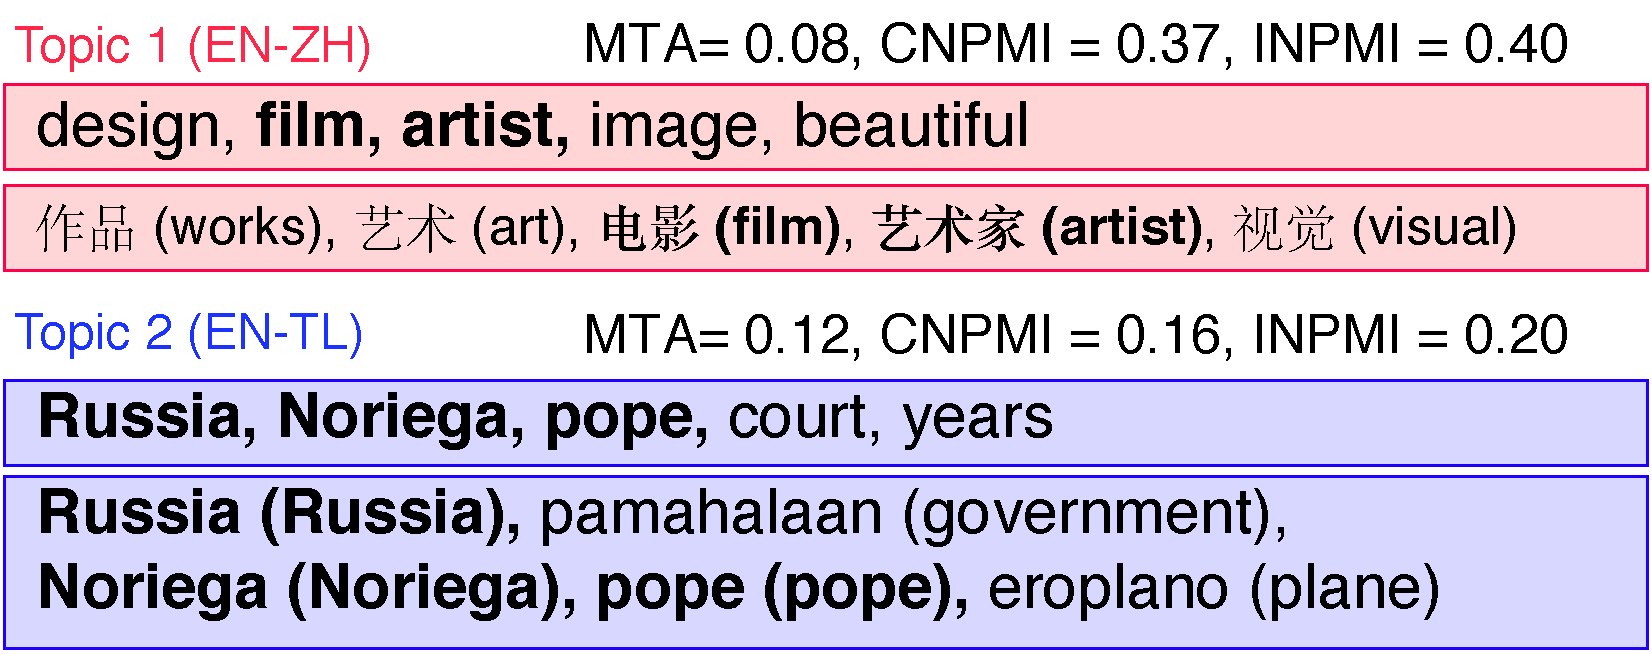
\includegraphics[width=\linewidth]{2018_naacl_mltm_eval/figures/mta_fail_example}
	\caption{\mta{} fails to capture semantically related words
          (Topic 1) and only looks at translation pairs regardless of
          internal coherence (Topic 2).}
	\label{fig:mtafailexample}
\end{figure}



\subsection{When \mta{} Falls Short}

We analyze \mta{} from two aspects---the inability to
capture semantically-related \textit{non-translation} topic words, and
insensitivity to cardinality---to show why \mta{} is not an ideal
measurement, even though it correlates well with human judgments.

\paragraph{Semantics}
We take two examples with \textsc{en-zh} (Topic 1) and \textsc{en-tl}
(Topic 2) in Figure~\ref{fig:mtafailexample}. Topic~1 has fewer
translation pairs than Topic~2, which leads to a lower \mta{} score
for Topic 1. However, all words in Topic 1 talk about \underline{art},
while it is hard to interpret Topic~2.  Wikipedia 
\cnpmi{} scores reveals Topic~1 is more coherent.  Because
our experiments are on datasets with little divergence between the
themes discussed across languages, this is uncommon for us but could
appear in noisier datasets.

\paragraph{Cardinality}  Increasing cardinality diminishes a topic's coherence~\cite{JHL16}.
We vary the cardinality of topics from ten to fifty at intervals of
ten (Figure~\ref{fig:add-card}).  As cardinality increases, more
low-probability and irrelevant words appear the topic, which lowers
\cnpmi{} scores.  However, \mta{} stays stable or increases with
increasing cardinality.  Thus, \mta{} fails to fulfill a critical
property of topic model evaluation.

\begin{figure*}[t]
  \centering
  \includegraphics{2018_naacl_mltm_eval/auto_fig/add_card_npmi_wiki}
  \includegraphics{2018_naacl_mltm_eval/auto_fig/add_card_npmi_bible}
  \includegraphics{2018_naacl_mltm_eval/auto_fig/add_card_npmi_mta}
	\caption{Increasing cardinality of topic pairs makes it harder
          to judge the coherence. Decreasing \cnpmi{} scores reflect
          the diminished interpretability of topics, while \mta{}
          scores do not.}
	\label{fig:add-card}
\end{figure*}

Finally, \mta{} requires a comprehensive multilingual dictionary,
which may be unavailable for low-resource languages.
Additionally,
most languages often only have one dictionary,
which makes it problematic to use the same resource (a
language's single multilingual dictionary) for training and evaluating
models that use a dictionary to build multilingual
topics~\cite{HuZEB14}.   Given these concerns, we continue the paper's focus on
\cnpmi{} as a data-driven alternative to \mta{}.  However, for many
applications \mta{} may suffice as a simple, adequate evaluation
metric.